\documentclass{article}
\usepackage[utf8]{inputenc}
\usepackage{amssymb}
\usepackage{amsmath}
\addtolength{\oddsidemargin}{-.875in}
\addtolength{\evensidemargin}{-.875in}
\addtolength{\textwidth}{1.75in}

\addtolength{\topmargin}{-1in}
\addtolength{\textheight}{1.75in}

\usepackage{graphicx}
\graphicspath{ {./Desktop/Notes/MA106} }

\title{MA106}
\author{Shubh Kumar}
\date{IIT-B, Spring Semester 2021}

\begin{document}

\maketitle

\section{Lecture 1: Introduction}
\begin{itemize}
    \item Matrices are a new universe of Numbers
    \item Visualizing the matrices as a column vector of row vectors or a row vector of column vectors, is an important thing
    \item Outer Product is called so, as its sort of doing the inner product/scalar product(or dot product!), the other way round!
    \item Going over the various ways to write the Product of Two Matrices

    \item Exercise: Proving Trivial Results like $\big(\textbf{AB}\big)^T$ = $\mathbf{B^{T}}$ $\mathbf{A^{T}}$

    \item The $j^{th}$ row of \textbf{AB} is a linear combination of the $j^{th}$ row of \textbf{A} with coefficient of some common, and analogically in case of $k^{th}$ column of \textbf{AB} would be
    \item Really Nice Question: Justifying the different cases of solutions to system of linear equations using concepts from matrices
\end{itemize}

\section{Lecture 2: Linear Systems}

\begin{itemize}
    \item General Linear system will include homogeneous as well as non-homogeneous.
    \item \textbf{Deducing Connections:} How to relate $\mathbf{Ax = b}$ to $\mathbf{Ax = 0}$. If $\mathbf{Ax = 0}$ has non-trivial solutions, than that would mean infinitely many solutions if we know just one solution exists.

    \item Extending the past concepts to more general cases: Using the above thing to solve any general system of m equations in n variables.

\end{itemize}

\section{Lecture 3: Gaussian Elimation}
Nothing as such apart from Lecture Notes introduced,
Just a very nice and thoughtful question:
Let $\mathbf{A} \in \mathbb{R}^{9x4}$ and $\mathbf{B} \in \mathbb{R}^{7x3}$. Is there $\mathbf{X}
\in \mathbb{R}^{4x7}$ such that $\mathbf{X} \ne \mathbf{O}$ but $\mathbf{AXB = O}$

\section{In General Observations/Queries which people posted on Whatsapp Group}
\begin{itemize}
  \item From LEC2, where first we identify the pivot points in REF, identify the free and non-free variables
  and then set the non-free ones to zero, following which we also identify the basis vectors by setting each one of
  them to one in and getting separate solutions, so that the overall solution is a linear combination of these.

  \item In the REF of an inconsistent System, we can get different REFs there is no unique one, but we do have
  a unique Reduced REF or Row-canonical Form.

  \item Another way to progress, after we've identified the Free variables in REF, would be to simply substitute
  the Free variables $x_i = \alpha_i$, but we don't do this, Why?

  \item 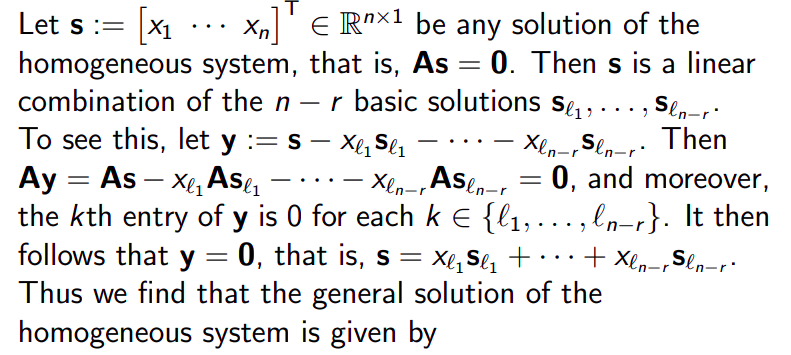
\includegraphics[scale = 0.5]{1.png} \\ Why is $\mathbf{y} = 0$ in the above paragraph?
  \item Try proving: For all $\mathbf{A} \in \mathbb{R}^{nxn}$ if  $\mathbf{AE=EA}$, for some $\mathbf{E} \in \mathbb{R}^{nxn}$
  such that $\mathbf{E = I}$.
  \item Let $I \subset \mathbb{R}^{n × n}$ be a nonempty set closed under addition such that $\mathbf{MN, NM} \in I $ whenever $\mathbf{N} \in I$ and $\mathbf{M} \in \mathbb{R}^{nxn}$. Show that either $I = 0$ or $I = \mathbb{R}^{nxn}$.
  \end{itemize}
\section {Lecture 4: Inverses and its usage in solving Linear Equations}
\begin{itemize}
  \item Try to prove: Let $\mathbf{A} \in \mathbb{R}^{nxn}.$iff $\mathbf{Ax = b}$ has only zero solution, then $\mathbf{A}$ is invertible
  \item Prove that for $\mathbf{A, B} \in \mathbb{R}^{nxn}$ such that $AB = I$, then $BA = I$.
  \item Lwt \textbf{A} and \textbf{B} be square matrices. Then \textbf{AB} is invertible iff \textbf{A} and \textbf{B} are invertible, and then $\mathbf{(AB)}^{-1} = \mathbf{B}^{-1}\mathbf{A}^{-1}.$

  \item Prove that every matrix has a unique Row-canonical form.
  \item Row Echelon Forms are never unique.

\end{itemize}

\section{Lecture 5: Inverses, Linear Dependence-Independence, Ranks}
\begin{itemize}
  \item The Gauss-Jordan Method provides us with the theoretical justification of what we used to do in 12th to find $\mathbf{A}^{-1}$ using EROs.
  \item If we aren't able to transform the matrix to $\mathbf{I}$ , then we'll get a row of 0s and will conclude that the matrix isn't invertible, and if we don't find any such row in any step, then we'll essentially end up getting the Identity Matrix and hence, the inverse.
  \item 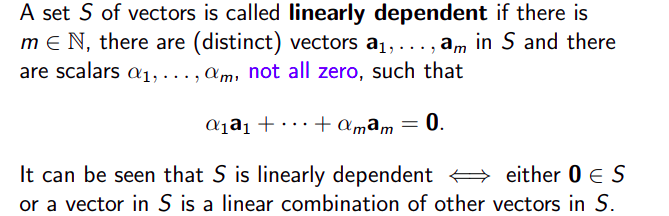
\includegraphics[scale = 0.5]{2.png} \\ Investigate meaning of the last line!
  \item 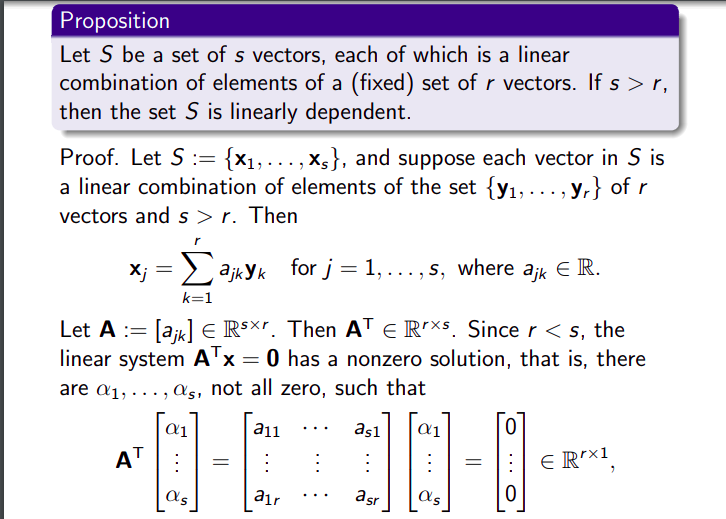
\includegraphics[scale = 0.5]{3.png} \\ This truly is an elegant proof, make various variations in the hypothesis condition and check why they are or aren't true.
  \item 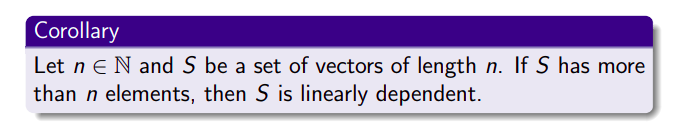
\includegraphics[scale = 0.5]{4.png} \\ Why this is so? Proof!
  \item Think of vectors which can be taken as a bunch of linearly-independent vectors which can be used as basis.
  \item A $nxn$ Square Matrix could be invertibe iff its rank is $n$.
  \item We can investigate linear-independence by simply taking some coefficients appropriately and see if
  it could possible give us non-trivial solutions, where not all of the coefficients are 0.

\end{itemize}

\section{Tutorial 2: Linear Dependency, Inverses}
\begin{itemize}
  \item A rectangular matrix can only have an inverse in certain cases, (By Inverse, I mean any matrix which when multiplied with our Matrix from one side, then that gives me $\mathbf{I}$!), Find out which ones these are, with legit mathematical arguements.
  \item  While, we can actually consider a lot of operations on matrices as elementary or its compositions, we follow the slides and consider only three basic cases:\\ 1) Exchanging Two Rows \\
  2) Adding the scalar multiple of one of the rows to another row \\ 3) Multiplying a particular row with a scalar.
  \item Together these operations bring us the concept of Elementary Matrices, each one of which can represent an Elementary Row Operation, (As in Q2.3!)
\end{itemize}
\section{Lecture 6: Rank, Subspaces, Basis and Span}
  \begin{itemize}
    \item While Calculating the Row Rank, which rows shall together form a set of linearly independent row vectors is an irrelevant question, as it depends on how we do our EROs, we may get a different set of such row vectors every time, but that won't matter, only the Rank would!
    \item An elegant technique to prove equality: Prove $a \leq b$ and $b \leq a$.
    \item Also, if there's an element of symmetry in proving $a \leq b$ and $b \leq a$, we only need to prove one and then exploit symmetry to claim the other.
    \item Exercise: Work out the size of the Subspace, if the basis of this subspace is consisting of $n$ vectors $\in \mathbb{R}^{nx1}$ in that space!
    \item Dimension of a Subspace is the same thing as the number of vectors in its basis.

  \end{itemize}

\section{Lecture 7: Column and Row Spaces, Determinants}

  \begin{itemize}
    \item Basis is the set of maximum number of independent vectors in a subspace.
    \item Basis could also be seen as the smallest spanning-set.
    \item If we have EROs, then that may change $\mathbf{C}(A)$, similarly, ECO could change $\mathbf{R}(A)$.
    \item Try Proving all Properties of Determinants.
    \item A Scalar Multiplication of 0, at any step of any ERO has no mearning!
  \end{itemize}

\end{document}
